\documentclass{article}
\usepackage[utf8]{inputenc} % - Defines what coding LaTeX uses. Use this one.
\usepackage{graphicx} % - Package for including images in the document.
\usepackage{amsmath}
\usepackage{mathtools}
\usepackage{gensymb}
\usepackage{float}
\usepackage{subfiles}
\usepackage{array}
\usepackage{tikz}
\usepackage{tikz-timing}
\usetikzlibrary{automata, positioning, arrows}
\usepackage{pgf-umlsd}
\usepackage[backend=biber]{biblatex}
\addbibresource{refs.bib}
\graphicspath{ {pictures/} } % - Path to where the images are located on your computer. In this case I have a folder (look to the left) "Images" where the images are gathered.


%%%%%%%%%%%%%%%%%%%%%%%%%%%%%%%%%%%%%%%%%%%%%%%%%%%%%%%%%%%%%%
% -               Title and affiliation                    - %
%%%%%%%%%%%%%%%%%%%%%%%%%%%%%%%%%%%%%%%%%%%%%%%%%%%%%%%%%%%%%%

\title{}

\author{}


\date{\today}

\begin{document}

\section{Theory}
Theory behind the design Arrowhead, SoS etc

\section{Problem formulation}
\label{sec:software:problem_formulation}

The problem solved by the software is to create a system according to the following high level functional requirements:\\
\begin{enumerate}
    \item A user can construct a mission for the robot to do some meaningful work.
    \item The mission can be sent to the robot and be executed in a way so the work is done.
    \item A higher priority mission can preempt a lower priority mission.
    \item Have a distributed, flexible and fault tolerant system.
\end{enumerate}

\section{Methods}

% software requirements.
% Design goals.
% Software design.

To solve the problem described in section \ref{sec:software:problem_formulation} the software from the group working on the snowblower in 2021 was first inspected. It was clear that it did not fullfil our requirements because it was not a distributed system but a monolith with some tightly coupled parts. Futhermore did it not have a flexible enough concept of a mission. Therefore was it decided to build a new system with a new design. This design is described in this section and the implementation is described in section \ref{sec:software:result}.

\subsection{Software system design}
\label{sec:software:design}

To be able to fulfill the first requirement a flexible mission construct is needed, a design for this construct is described in section \ref{sec:mission}. To then be able to execute this mission a system of systems (SoS) was designed and described in section \ref{sec:software:sos_design}. After this each system is described section \ref{sec:software:first} to \ref{sec:software:last}.

\subsubsection{The mission construct}
\label{sec:mission}

A mission is constructed as a series of simple tasks that the robot is to carry out to accomplish some work.
For example if the robot have a snowblower accessory attached and we want it to carry out the work of clearing a area of snow a mission like this could be constructed:
\begin{enumerate}
    \item SET ACCESSORY TILT: to 100\%.
    \item GOTO: starting point.
    \item SET ACCESSORY TILT: to 0\%.
    \item ACCESSORY COMMAND: hold shute at $30^o$.
    \item ACCESSORY COMMAND: start blower.
    \item FOLLOW PATH: plow area path.
    \item ACCESSORY COMMAND: stop hold shute.
    \item ACCESSORY COMMAND: stop blower.
\end{enumerate}
In this example mission, first the accessory is tilted up to lift it upp as much as possible.
Then it goes to the starting point. After this it tilts down the accessory, tells the accessory to hold the shute at a angle so the snow is moved to a optimal spot and start the blower.
After the accessory is set up it follows a path that covers the area. When it's done clearing the snow it turns of the parts of the accessory it turned on.
This shows how a mission can be constructed using a list of tasks.

The type of tasks that can be used is given an overview in table \ref{tab:task_types_over}.
\begin{table}[H]
    \centering
    \begin{tabular}{| m{3cm} | m{5cm} |}
        \hline
        Task type & Description \\
        \hline \hline
        GOTO & Move the robot to a specific GPS point. \\
        \hline
        FOLLOW PATH & Make the robot follow a path represented as a list of GPS points. \\
        \hline
        WAIT & Wait for a set amount of time. \\
        \hline
        ACCESSORY COMMAND & Send a command to the accessory. \\
        \hline
        SET ACCESSORY TILT & Tilt the accessory a percentage where 100\% is as furthest from the ground and 0\% is closest to the ground. \\
        \hline
    \end{tabular}
    \caption{Overview of task types.}
    \label{tab:task_types_over}
\end{table}

\subsubsection{System of Systems design}
\label{sec:software:sos_design}

\begin{figure}[H]
    \includegraphics[width=\textwidth]{software_overview.png}
    \caption{Overview of the software architecture.}
    \label{fig:software_overview}
\end{figure}

The design of the software system is made up of different parts and are shown in figure \ref{fig:software_overview}. 
In figure \ref{fig:software_overview} each system is symbolized by a square with a describing name and
lines symbolize communication between systems. Some communication lines are omitted for clarity.

The design was divided into 4 main parts, each part has its own color in figure \ref{fig:software_overview}:

The safety critical part is shown in blue and controls the robot directly. This part is described in section (? ref to other Eriks part ?). The part communicate with the rest of the system over a UART \cite{IEEEUART} link with the Robot control interface system.

The non safety critical part is shown in the green big rectangle.
This part handles everything needed to do to carry out a mission and sends the proper commands to either the robot controller or the accessory.

The red part is the accessory, it controls the accessory directly.
The accessory is designed to be able to be any kind of accessory. In our test case it is a snowblower.

The last part in light green in the little cloud is running on a server somewhere. It is designed to be the interface between the robot and the world being able to get telemetry from the robot and send missions for it to do.

The green and red parts systems are arrowhead framework systems \cite{delsing2017arrowhead} running in a local cloud on the robot. By using the arrowhead framework these systems must each communicate with each other true well defined application programming interfaces (API). With these APIs a system can easily be changed out with another system implementing the same API or even more then one system implementing each implementing a part of the API.
The arrowhead framework also provides late binding between systems, witch means that a system only need to know the address of a service it needs to use when it actually want to use it at runtime.
To facilitate this late binding each arrowhead local cloud needs to have a set of core systems \cite{varga2017making}.

The systems in the cloud down to the right in figure \ref{fig:software_overview} is run in a separate arrowhead local cloud with it's own set of core systems. To be able to communicate with the other local cloud the gateway optional core system \cite{varga2015service} was used.

\begin{figure}
\centering
        \resizebox{\textwidth}{!}{
        \begin{sequencediagram}
            \newthread{plan}{Mission planner}
            \newthread{schedule}{Mission scheduler}
            \newinst[3]{exec}{Mission executor}
            \newinst{gps}{GPS interface}
            \newinst{vision}{Vision system}
            \newinst{nav}{Navigation system}
            \newinst{robot}{Robot control interface}
            \newthread{bat}{Battery estimator}

            \mess{plan}{Add some mission}{schedule}
            \begin{call}
                {schedule}{Do some mission}{exec}{Done}
                \begin{call}
                    {exec}{Navigate to point}{nav}{Aborted}
                    \begin{call}
                        {nav}{Get coordinates}{gps}{Coordinates}
                    \end{call}
                    \begin{call}
                        {nav}{Set track speeds}{robot}{}
                    \end{call}
                    \begin{call}
                        {nav}{Get coordinates}{gps}{Coordinates}
                    \end{call}
                    \begin{call}
                        {nav}{Set track speeds}{robot}{}
                    \end{call}
                    \mess{bat}{Add charge mission}{schedule}
                    \mess{schedule}{Do charge mission}{exec}
                    \mess{exec}{Abort}{nav}
                \end{call}
                \mess{exec}{Add reminder of some mission}{schedule}
                \begin{call}
                    {exec}{Navigate to charger}{nav}{Done}
                    \begin{call}
                        {nav}{Get coordinates}{gps}{Coordinates}
                    \end{call}
                    \begin{call}
                        {nav}{Get direction}{vision}{Not visible}
                    \end{call}
                    \begin{call}
                        {nav}{Set track speeds}{robot}{}
                    \end{call}
                    \begin{call}
                        {nav}{Get coordinates}{gps}{Coordinates}
                    \end{call}
                    \begin{call}
                        {nav}{Get direction}{vision}{Direction}
                    \end{call}
                    \begin{call}
                        {nav}{Set track speeds}{robot}{}
                    \end{call}
                \end{call}
            \end{call}
            \begin{call}
                {schedule}{Do remainder of some mission}{exec}{Done}
                \begin{call}
                    {exec}{Navigate to point}{nav}{Aborted}
                    \begin{call}
                        {nav}{Get coordinates}{gps}{Coordinates}
                    \end{call}
                    \begin{call}
                        {nav}{Set track speeds}{robot}{}
                    \end{call}
                    \begin{call}
                        {nav}{Get coordinates}{gps}{Coordinates}
                    \end{call}
                    \begin{call}
                        {nav}{Set track speeds}{robot}{}
                    \end{call}
                \end{call}
            \end{call}
        \end{sequencediagram}
        }
    \caption{Sequence diagram for snowblower robot systems executing a mission and then interrupt it with a charge mission.}
    \label{fig:sequence2}
\end{figure}

To show how the systems may work together a sequence diagram is shown in figure \ref{fig:sequence2}.
In the sequence diagram the robot first do a mission where it navigates to a point and is preempted by a higher priority mission to charge the robot.
The way preemption is handled is that the mission executor when it's get a new mission will construct a new mission that will carry out the work left on the current mission and send this new mission to the mission scheduler.

\subsection{Accesory control}
\label{sec:software:first}
The accessory control system takes accessory commands and carries them out by controlling the accessory.
What accessory commands ara available depend on the accessory and each accessory type need its own accessory control.
To be able to know what accessory is attached a get accessory type service is provided and to validate that the command can be interpreted by the specific accessory controller the accessory type is sent alongside each command.

\subsection{Battery estimator}
The battery estimator gets information battery from the robot control interface and estimates battery life left.
When the battery life left is to short it can issue a high priority go charge mission if appropriate.

\subsection{GPS interface}
The GPS interface gets information from the GPS unit and makes it available to the other systems thru provided services.

\subsection{Mission executor}
The mission executor handles the execution of the missions. When its do mission service is consumed it will take the mission and for each task send the right service request with the right data. It can be looked upon as a translator between mission task and service request.
It also sends a add mission request to the mission scheduler with a mission that will do the remaining work of a mission interrupted by another mission to enable preemption.

\subsection{Mission scheduler}
The mission scheduler as the name implies schedules the missions. It schedules the mission by highest priority first and if same priority oldest first.
The function of the mission scheduler can be described by the state diagram shown in figure \ref{fig:mission_scheduler_state}.
When in the send mission state either the new mission or the first mission in the queue is sent to the mission executor.
\tikzset{
->, % makes the edges directed
node distance=6cm, % specifies the minimum distance between two nodes. Change if necessary.
every state/.style={thick, fill=gray!10}, % sets the properties for each ’state’ node
initial text=$ $, % sets the text that appears on the start arrow
}
\begin{figure}
    \centering
    \resizebox{16cm}{!}{
    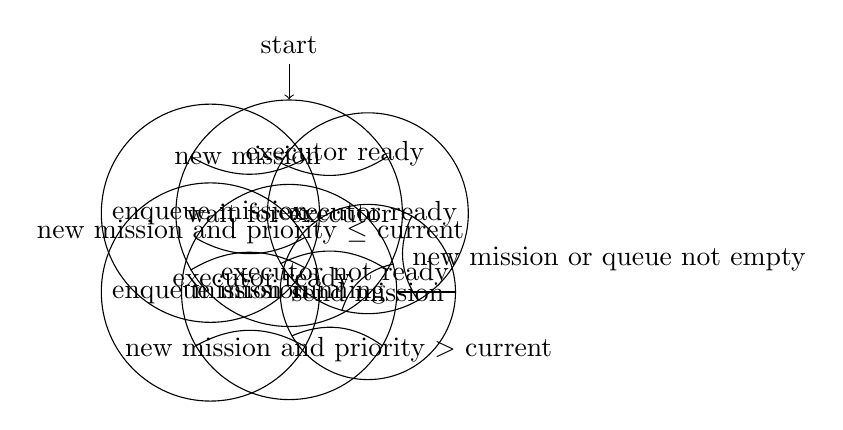
\begin{tikzpicture}
        \node[state, initial, initial where=above] (wait) {wait for executor};
        \node[state, right of=wait] (ready) {executor ready};
        \node[state, below of=ready] (send) {send mission};
        \node[state, left of=wait] (enqueue1) {enqueue mission};
        \node[state, below of=wait] (running) {mission running};
        \node[state, left of=running] (enqueue2) {enqueue mission};

        \draw
        (wait) edge[bend left, above] node{executor ready} (ready)
        (ready) edge[bend left, below] node{executor not ready} (wait)
        (wait) edge[bend right, above] node{new mission} (enqueue1)
        (enqueue1) edge[bend right, left] node{} (wait)
        (ready) edge[bend left, right] node{new mission or queue not empty} (send)
        (send) edge[] node{} (running)
        (running) edge[bend right, above] node{new mission and priority $\leq$ current} (enqueue2)
        (running) edge[bend right, below] node{new mission and priority $>$ current} (send)
        (enqueue2) edge[bend right] node{} (running)
        (running) edge[left, bend right] node{executor ready} (ready)
        ;
    \end{tikzpicture}
    }
    \caption{State diagram for mission scheduler.}
    \label{fig:mission_scheduler_state}
\end{figure}

\subsection{Navigator}
The navigator navigate the robot by getting position and heading from the GPS interface or a relative heading and distance from the Vision system and comparing it to where it should be send the appropriate track speeds to the robot control interface. It can receive either a GPS point to navigate to, a path represented by a list of GPS points to follow or a marker id to navigate to.

\subsection{Robot control interface}
The robot control interface communicates with the safety critical system that directly controls the robot. It can receive requests to set the track speeds, tilt accessory etc.

\subsection{Stopper system}
The stopper system sends stop requests to all applicable systems when it receives a stop request.

\subsection{Telemetry collector}
The telemetry collector collects telemetry from most other system to relay it to the user via for example a web interface running on some server somewhere.

\subsection{Vision system}
\label{sec:software:last}
The vision system is connected to stereo cameras.
It uses the cameras to identify when something is to close in front of the robot and stop it by a request to the stopper system.
Other then identifying obstacles it can also get the distance and bearing to a fiduciary marker.
For more information about the camera system se section (? ref to Antons part ?).

\section{Result}
\label{sec:software:result}

To validate the design described in section \ref{sec:software:design} it was implemented.
The arrowhead systems where implemented in Java using a arrowhead application library \cite{arrowheadlib}.
For the core system of the arrowhead local cloud core-java-spring \cite{arrowheadcore} was used.
Due to time limitations was not the entire design implemented and only the local cloud on the robot was set up.
Table \ref{tab:implementation_status} shows the status of completeness for each system implementation. To test the parts of the system that where done a mission that started with a go to point task then a follow path task and finally another go to point task was sent to the mission scheduler. After this the robot first navigated to the point then followed the path and finally navigated to the point showing that the mission scheduler, mission executor, navigator, GPS interface and robot control interface for this case worked as intended.
\begin{table}
    \centering
    \begin{tabular}{|l|p{8cm}|}
        \hline
        System & Implementation status \\
        \hline
        \hline
        Accessory control & Initial version written but not tested and integrated. \\
        \hline
        Battery estimator & Nothing done. \\
        \hline
        GPS interface & Done apart from telemetry. \\
        \hline
        Mission executor & Done for follow path and go to point tasks, no telemetry or mission reconstruction on interruption. \\
        \hline
        Mission scheduler & Done apart from telemetry. \\
        \hline
        Navigator & Done for go to point and follow path. \\
        \hline
        Robot control interface & Done for set track speeds. \\
        \hline
        Stopper system & Nothing done. \\
        \hline
        Telemetry collector & Nothing done. \\
        \hline
        Vision system & Not fully tested and implemented with arrowhead. \\
        \hline
    \end{tabular}
    \caption{Implementation status of all the systems.}
    \label{tab:implementation_status}
\end{table}

\section{Discussion}
As shown in section \ref{sec:software:result} a mission was able to be constructed that did meaningful work in this case moving the robot around so the first and second requirement was met. For the third requirement the design was done to enable thru the mission executor adding a new mission for the work left to do in the interrupted mission to the mission scheduler. 
This was not implemented as seen in table \ref{tab:implementation_status} so is to be seen how well this works in practice.
When it comes to the fourth requirement it is hard to say wether or not the design fulfill it. Altho the design is clearly distributed and parts of the distributed system was shown to work in practice. Furthermore was the system made to be fault tolerant by separating the system into safety critical and non safety critical parts. By doing this the safety critical system can ignore the instruction from the non safety critical system if an operator turn a switch on the remote. The flexible part of the requirement is somewhat fulfilled by having a system of systems with well defined APIs whish enables a system to be changed out to another system that implement the same API.

\section{Conclusion}
To conclude was the requirements met even thou many features are missing from the implementation.

\printbibliography


\end{document}